\section{Methodology}

\subsection{Data Cleaning and Preprocessing}

This study uses data from Crunchbase, a commercial database that has emerged as a primary source for entrepreneurship and venture capital research \cite{OECD2017}. Founded in 2007 as a side project to TechCrunch, Crunchbase has evolved into a crowdsourced platform containing detailed information about startups, venture capital firms, accelerators, and investment rounds globally. The platform relies on multiple data collection methods, including user submissions, automated web crawling, partnerships with data providers, and editorial curation \cite{OECD2017}.

The dataset was obtained by querying Crunchbase for all investment transactions involving enterprises (startups, scale-ups, and growth companies) domiciled in the United States, which captures the complete investment ecosystem for US-based firms, including both domestic and cross-border capital flows. 

Foreign venture capital firms and institutional investors appear in the dataset when they participate in financing rounds of US enterprises. Furthermore, Crunchbase's coverage is particularly good for technology-oriented startups and venture capital transactions, making it well-suited for studies of innovation ecosystems and investment networks.

However, limitations and potential biases must be acknowledged when using Crunchbase data \cite{OECD2017}, for instance:

\begin{itemize}
    \item \textbf{Geographic bias}: Stronger coverage of US and Western European markets compared to emerging economies.
    \item \textbf{Sectoral bias}: Emphasis on technology and internet companies, potentially underrepresenting traditional industries.
    \item \textbf{Venture capital bias}: Better documentation of VC-backed companies compared to bootstrapped or debt-financed ventures (which may not be problematic for this study).
    \item \textbf{Size bias}: Larger and more successful companies are more likely to be thoroughly documented.
    \item \textbf{Temporal bias}: More recent information tends to be more complete and accurate than historical records.
\end{itemize}

These biases do not invalidate research using Crunchbase but require careful consideration in study design and interpretation of results. For network analysis of venture capital co-investments, the VC bias may actually enhance data quality by focusing on the target population of interest.

The data preprocessing and cleaning follows established methodologies from entrepreneurship literature \cite{Dalle2025} and is implemented through the following multi-step procedure:

\begin{enumerate}
    \item \textbf{Company data cleaning}: Removal of companies with incomplete essential information (missing unique identifiers, names, or founding years), exclusion of companies founded after 2017 to allow sufficient time for investment patterns to emerge, and removal of companies with exit status (closed, acquired, or IPO).
    
    \item \textbf{Investment data cleaning}: Removal of investment records with missing essential linkage information (company or investor identifiers), elimination of investments with invalid funding amounts (negative or zero values), and validation of funding consistency by excluding rounds where the sum of individual investments does not match the total funding amount reported in the database.
    
    \item \textbf{Funding threshold application}: Restriction of the sample to companies that raised more than \$150{,}000 in total funding to focus on substantive investment relationships and ensure stronger statistical reliability.
    
    % \item \textbf{Endogeneity bias prevention}: Exclusion of companies that received funding exclusively from accelerators or incubators to prevent endogeneity bias, as these companies may not have attracted independent market validation from external investors.
    
    \item \textbf{Data consistency validation}: Final consistency checks to ensure all investment records reference existing companies in the dataset and all retained companies have at least one valid investment record.
\end{enumerate}

\subsection{Network Construction}

The network construction process transforms raw investment data into a structured bipartite representation that enables theoretical reasoning about venture capital syndication patterns. This transformation follows the conceptual framework outlined by \cite{Borgatti2011}, who distinguish between flow models (focusing on how resources move through networks) and bond models (emphasizing coordination and solidarity among actors).

The construction process involves three sequential transformations, each representing a different conceptualization of network ties, each one described in \ref{fig:bipartite_pipeline} and in the subsequent paragraphs below.

\begin{figure}[htbp]
    \centering
    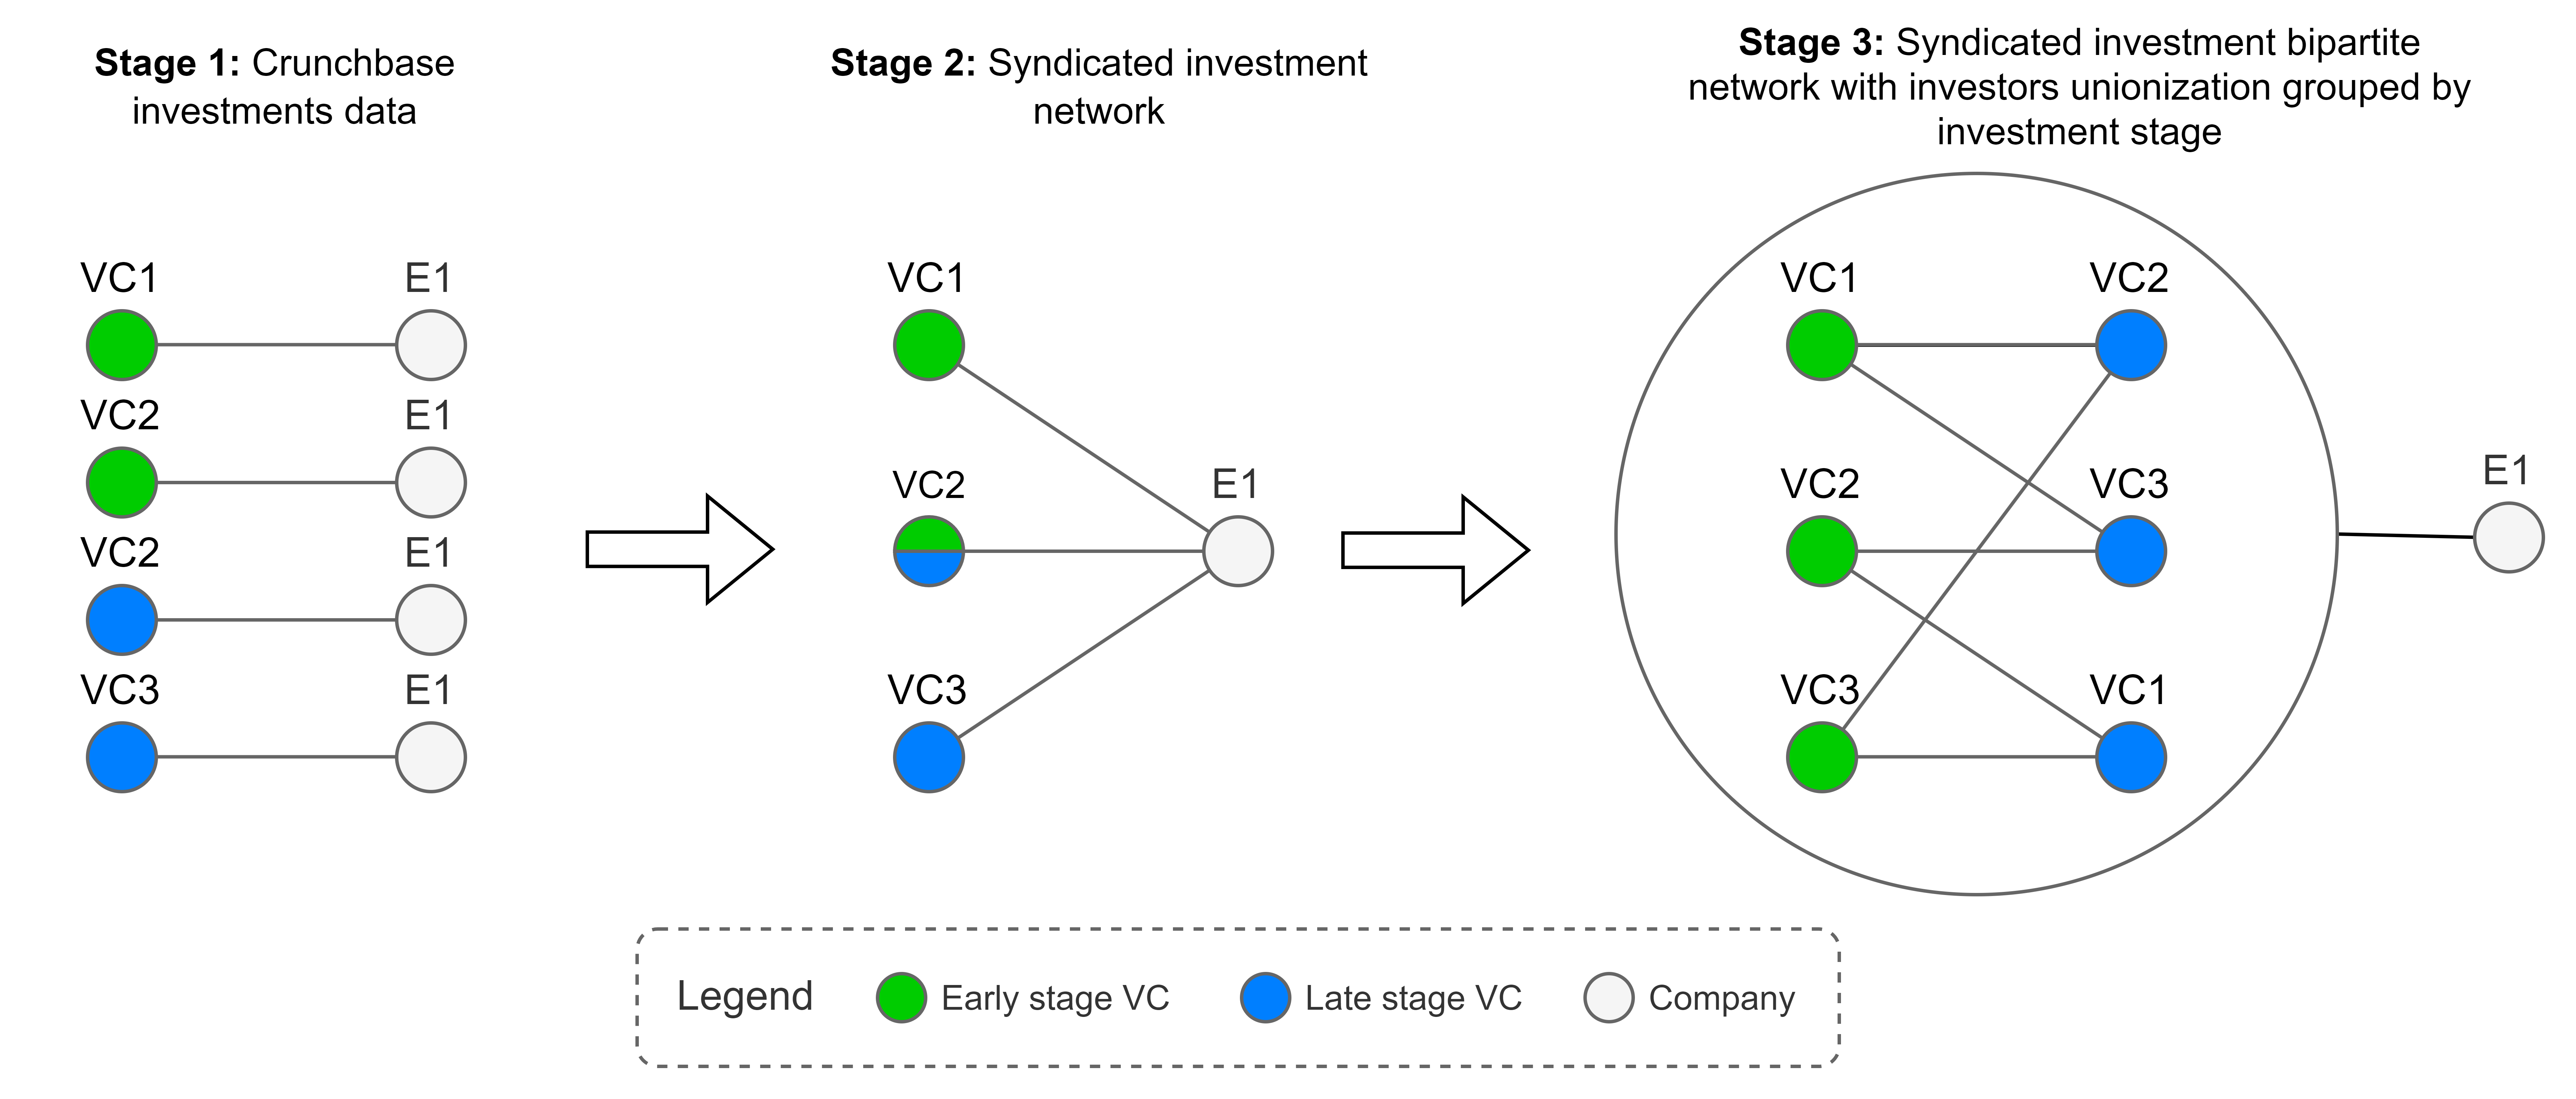
\includegraphics[width=\textwidth]{../diagrams/vc_investment_bipartite_pipeline.png}
    \caption{From event-type investment ties to bipartite syndicate networks: structuring vc relations through flow and bond models}
    \label{fig:bipartite_pipeline}
\end{figure}

\textbf{Stage 1 - Raw event-type investment ties:}
The initial Crunchbase dataset records discrete transactional relationships between venture capital firms and portfolio companies. These event-type ties represent what \cite{Borgatti2011} characterize as nominalist network constructions, where investment transactions ere defined as the fundamental tie type that constitutes the network in that stage. Each investment event creates a direct dyadic relationship between a venture capital firm and a company, but these isolated ties do not yet reveal the broader structural patterns of co-investment behavior.

\textbf{Stage 2 - Syndicated investment network construction:}
The raw event data are aggregated to identify co-investment relationships, where multiple venture capital firms participate in the same funding round or invest in the same company across different rounds. This aggregation transforms discrete investment events into a network structure where venture capital firms become indirectly connected through their shared ties to portfolio companies. Following \cite{Borgatti2011}, this step creates pathways between actors that enable analysis of their relative positions, including measures of centrality and brokerage within the investment ecosystem.

\textbf{Stage 3 - Bipartite network segmentation by investment stage:}
The final transformation reorganizes the syndicated network into a bipartite structure that separates investors based on their participation in different funding stages. 

First, investment stages are categorized into two main groups:
\begin{itemize}
    \item Early stages: angel, pre-seed, seed, and Series A
    \item Late stages: Series B through Series I
\end{itemize}

This bipartite structure reflects both flow and bond models as described by \cite{Borgatti2011}. The flow model perspective enables analysis of how resources and information traverse across investment stages, capturing the sequential nature of venture capital financing. Simultaneously, the bond model perspective recognizes that co-investors within each stage can be conceptualized as forming coordinated coalitions, reflecting solidarity ties among investors.

An important consideration in this construction involves investors who participate in both early and late stages (for example, a venture capital firm that invests in both Series A and Series C rounds). In such exceptional cases, the same investor appears as distinct agents on both sides of the bipartite network. This separation is achieved by appending the investment stage identifier to the unique investor UUID during the network construction process, effectively creating stage-specific identities for multi-stage investors. This approach ensures that the bipartite structure remains mathematically valid while preserving the analytical ability to study how the same investor behaves differently across investment stages.

The resulting bipartite graph connects two distinct sets of investors: those participating in early-stage rounds and those participating in late-stage rounds. Edges represent co-investment relationships where early-stage and late-stage investors have both invested in the same company, creating a bridge between different phases of the venture capital investment cycle.

Formally, the bipartite graph $G = (U \cup V, E)$ consists of:
\begin{align}
U &= \{u_1, u_2, \ldots, u_m\} \text{ (late-stage VCs)} \\
V &= \{v_1, v_2, \ldots, v_n\} \text{ (early-stage VCs)} \\
E &\subseteq U \times V \text{ (co-investment relationships)}
\end{align}

To prevent spurious connections from related entities, investor pairs where the first five characters of their names match are filtered out, reducing the likelihood of including different funds from the same parent organization. Furthermore, investors that participated in both early and late stages receive a suffix so they can be treated as distinct agents for each phase.

\subsection{Community Detection}

Community structure in the bipartite network is identified using modularity-based optimization methods, building on foundational work by \cite{Newman2006} who established modularity as a key metric for community detection in complex networks. For bipartite networks specifically, we employ the greedy modularity optimization algorithm following \cite{Barber2007}, who introduced a modularity definition tailored for bipartite graphs and developed corresponding algorithms that account for the distinct node sets characteristic of bipartite structures.

The choice of greedy optimization is motivated by its computational efficiency and scalability, as demonstrated by \cite{Blondel2008} in their widely-adopted Louvain algorithm. This approach iteratively merges communities to maximize the modularity score, which measures the density of connections within communities compared to connections between communities.

For a bipartite network, modularity $Q$ is defined as:
\begin{equation}
Q = \frac{1}{2m} \sum_{i,j} \left[ A_{ij} - \frac{k_i k_j}{2m} \right] \delta(c_i, c_j)
\end{equation}

where $A_{ij}$ is the adjacency matrix, $k_i$ is the degree of node $i$, $m$ is the total number of edges, $c_i$ is the community of node $i$, and $\delta(c_i, c_j)$ is 1 if nodes $i$ and $j$ are in the same community, 0 otherwise.

This methodology has proven particularly effective in venture capital research, as demonstrated by \cite{Bubna2020} who used computational methods over three decades of syndication data to identify venture capital communities. Their work establishes empirical precedent for applying community detection algorithms to co-investment networks, showing that such methods can reveal meaningful structural patterns in the investment ecosystem that may not be apparent from individual investment decisions.

\subsection{Nestedness Analysis}

Nestedness is a structural property commonly observed in ecological networks \cite{AlmeidaNeto2008} that describes the tendency for specialists to interact with a subset of the partners of generalists. In the context of venture capital networks, nestedness would indicate that investors with fewer connections tend to co-invest with a subset of the partners of more connected investors.

We measure nestedness using the NODF (Nestedness based on Overlap and Decreasing Fill) metric \cite{AlmeidaNeto2008}, which has become a standard measure for quantifying nested patterns in bipartite networks. The NODF metric is particularly well-suited for network analysis as it provides a standardized measure that accounts for both the overlap of connections and the degree differences between nodes \cite{Dormann2009}.

For a bipartite adjacency matrix $M$ with rows and columns sorted by decreasing degree, NODF is calculated as:

\begin{equation}
NODF = \frac{NODF_{rows} + NODF_{columns}}{2}
\end{equation}

where:
\begin{align}
NODF_{rows} &= \frac{100}{R(R-1)/2} \sum_{i=1}^{R-1} \sum_{j=i+1}^{R} \frac{|N_i \cap N_j|}{k_j} \text{ if } k_i > k_j \\
NODF_{columns} &= \frac{100}{C(C-1)/2} \sum_{i=1}^{C-1} \sum_{j=i+1}^{C} \frac{|N_i \cap N_j|}{k_j} \text{ if } k_i > k_j
\end{align}

Here, $R$ and $C$ are the number of rows and columns, $N_i$ represents the set of connections for node $i$, and $k_i$ is the degree of node $i$.

Using this method, NODF values range between 0 and 1 (perfect nestedness).

\subsection{Statistical Significance Testing}

To determine whether observed nestedness values differ significantly from what would be expected by chance, we employ a null model approach using the Curveball algorithm \cite{Strona2014}. This algorithm generates randomized matrices that preserve the degree sequence of both node sets while randomizing the connection patterns, representing a "hard" constraint null model that maintains structural properties while randomizing interaction patterns \cite{Dormann2009}.

The choice of degree-preserving null models is critical for nestedness interpretation, as the degree sequence itself can influence apparent nestedness patterns. By preserving degree sequences, we ensure that observed nestedness reflects genuine structural organization rather than mere consequences of heterogeneous node connectivity.

For each community, we generate 100 null matrices using 10,000 Curveball iterations. The statistical significance is assessed by comparing the observed NODF score against the distribution of null model scores:

\todo[inline]{Generate 1000 null matrices instead}

The standardized Z-score is calculated to quantify how many standard deviations the observed nestedness differs from the null expectation:

\begin{equation}
Z = \frac{NODF_{observed} - \mu_{null}}{\sigma_{null}}
\end{equation}

where $\mu_{null}$ and $\sigma_{null}$ are the mean and standard deviation of the null distribution, respectively.

The p-value is calculated empirically from the null distribution as the proportion of randomized matrices that exhibit nestedness equal to or greater than the observed value:

\begin{equation}
p = \frac{1 + \sum_{i=1}^{N} I(NODF_{null,i} \geq NODF_{observed})}{N + 1}
\end{equation}

where $N$ is the number of null matrices (100 in our case), $NODF_{null,i}$ is the nestedness score of the $i$-th null matrix, and $I(\cdot)$ is an indicator function that equals 1 when the condition is true and 0 otherwise. The addition of 1 in both numerator and denominator provides a conservative estimate that avoids p-values of exactly zero.

The p-value represents the probability of observing nestedness as high as or higher than the observed value under the null hypothesis of random co-investment patterns. Communities with $p < 0.05$ are considered to have significantly high nestedness (when observed values exceed null expectations) or significantly low nestedness (when observed values fall below null expectations), indicating that the observed nested structure is unlikely to have arisen by chance alone.

While both Z-scores and p-values assess statistical significance, they provide complementary information: the Z-score quantifies the magnitude of deviation from the null expectation in standardized units, while the p-value provides the probability of observing such deviation under the null hypothesis. In our analysis, we primarily rely on p-values for significance testing as they directly quantify the statistical evidence against the null hypothesis of random network structure.
